\section{Evaluation}

In diesem Kapitel geht es um die Evaluation der Arbeit. Dies ist im doppelten Sinne zu verstehen: Einerseits soll der erstellte Prototyp anhand verschiedener Metrtiken (siehe \secref{sec:evaluationsmetriken}) evaluiert werden (technische Evaluation); andererseits soll das Ergebnis der Arbeit in einem übergeordneten Kontext, der auch den vorliegenden Bericht umfasst, im Bezug auf die Zielerreichung (siehe \secref{sec:projektauftrag}) evaluiert und reflektiert werden (Evaluation des Zielerreichung).

\subsection{Technische Evaluation}
\label{sec:technische-evaluation}

Der erstellte Protoyp kombiniert drei bestehende Modelle bzw. drei Arten von Modellen zu einem Gesamtsystem, das gegen aussen den Eindruck erweckt, als würde nur eine Art von Prediction erstellt: das Scoring der Gelenke. Das Erkennen des Körperteils und die Extraktion der Bildausschnitte, welche die Gelenke zeigen, ist für den Endanwender transparent.

Für die einzelnen Modelle (\texttt{body\_part}, \texttt{joint\_detection} und \texttt{ratingen\_score}) gibt es teilweise bereits Evaluationsmechanismen. Diese wurden im Rahmen der Entwicklung der einzelnen Modelle erstellt. Soll ein einzelnes Modell verbessert werden, ist dieses isoliert im Rahmen dieses Vorgangs zu evaluieren.

Im Rahmen der vorliegenden Arbeit soll es nur um die Evaluation des Gesamtsystems gehen. Wird ein bestehendes Modell verbessert, hat dies Einfluss auf die Performance des Gesamtsystems. Diese Verbesserung soll mit einem Evaluationsworkflow ermittelt werden können. Dieser kann dabei behilflich sein, den Fokus für die Verbesserung bestehender Modelle richtig zu legen, sodass man Aufwand in diejenigen Modelle steckt, deren Verbesserung einen Performancegewinn für das Gesamtsystem bedeuten.\footnote{Mit \textit{Performance} ist in diesem Kontext v.a. die Qualität der Predictions gemeint. Betreffend Laufzeitperformance wären Verbesserungen am Modell \texttt{joint\_detection} jedoch auch sehr wünschenswert.}

Da die Modelle im laufenden Betrieb nicht weitertrainiert werden, bietet sich eine \textit{Off\-line-Evaluation} an. Für die Offline-Evaluation eines Modells (bzw. eines Systems von Modellen) gibt es verschiedene Varianten: \textit{Hold-Out Validation}, \textit{Cross-Validation}, \textit{Bootstrapping} \cite[S. 19]{zheng2015}. Die Hold-Out Validation ist eine einfache Variante, erfordert aber ein zusätzliches Evaluationsdatenset, das einerseits unabhängig von und andererseits gleich verteilt wie das Trainingsdatenset sein muss (i.i.d.: \textit{independently and identically distributed}).\footnote{Ob die \textit{i.i.d.}-Hypothese für das Test- und das Evaluationsdatenset zutrifft, soll nicht im Rahmen der vorliegenden Arbeit geprüft werden. Die Problematik wird in \secref{sec:ungeloeste-probleme} erläutert.}

\subsubsection{Evaluationsdaten}
\label{sec:evaluationsdaten}

Als Quelle für die Trainingsdaten aller involvierter Modelle diente die SCQM-Datenbank. Für das Trainieren der Modelle wurden umfassende Datensätze daraus verwendet. In der Zwischenzeit ist die SCQM-Datenbank weiter angewachsen, sodass es eine signifikante ‒ und wichtiger: stetig wachsende ‒ Anzahl neuer Testdaten gibt, die zum Zeitpunkt der Erstellung der Modelle noch nicht vorhanden waren. Da die Modelle auf das Jahr 2018 (und früher) zurückgehen, können die Daten ab dem 1. Januar 2019 für die Evaluation verwendet werden. Diese wurden noch von keinem der drei Modelle «gesehen».

Für die Auswahl der Evaluationsdaten wurden vom Auftraggeber zwei CSV-Dateien zur Verfügung gestellt\footnote{Diese Dateien befinden sich aus Gründen des Datenschutzes nicht im Abgabeordner.}: Die eine enthält u.a. die eigentlichen Scores mit Datumsangaben und Referenzen auf die zugrundeliegende Studie. Die andere erhält Informationen zu den Studien, u.a. auch die Referenz auf den Patienten. Die Informationen aus den beiden Dateien müssen kombiniert werden\footnote{Dies wurde mit dem Python-Skript \texttt{deepxray/test\_data\_selection/extract.py} bewerkstelligt}, um so die Dateinamen ableiten zu können. Aufgrund dieser Selektion konnten vom Auftraggeber 1619 Röntgenbilder zur Verfügung gestellt werden, die jedoch verschiedene Körperteile zeigen.

Es musste somit eine Selektion vorgenommen werden, sodass im Evaluationsdatenset nur Röntgenbilder linker Hände zu finden sind. Anhand der Metadaten (erwähnte CSV-Dateien) ist dies leider nicht möglich. Eine Selektion anhand der Scores (mindestens eine Score von MCP1-5 oder PIP1-5 ungleich null) ist auch nicht möglich, da die SCQM-Datenbank auch Bilder gesunder Hände enthält. Die Selektion hatte darum manuell zu erfolgen. Um den mechanischen Vorgang der Kategorisierung von 1619 Röntgenbildern ‒ zeigt es eine linke Hand oder ein anderes Körperteil? ‒ komfortabler vornehmen zu können, wurde ein Python-Skript geschrieben, womit sich die Bilder interaktiv kategorisieren lassen.\footnote{Siehe \texttt{deepxray/test\_data\_selection/categorize.py}. Das Skript arbeitet die CSV-Datei ab, die alle Scores und Dateinamen enthält. Jedes Bild wird in Firefox in einem neuen Tab geöffnet. Dabei wandert der Fokus \textit{nicht} auf ein anderes Fenster, sondern bleibt auf der Kommandozeile. Zeigt das Bild eine linke Hand, kann \texttt{a} (wie «accept») und \texttt{[Return]} eingegeben werden, um die Zeile aus der CSV-Datei sowie das Bild zu übernehmen. Gibt man nur \texttt{[Return]} ein, werden Bild und CSV-Zeile verworfen.} Auf diese Weise konnten von den ursprünglichen 1619 Röntgenbildern 290 Aufnahmen linker Hände selektiert werden.

Die CSV-Dateien enthalten zu jedem Bild die Scores aller relevanter Gelenke (MCP 1-5, PIP 1-5). Diese Scores liegen in Prozentangaben vor. Da der Prototyp, bzw. das zugrundeliegende Modell \texttt{ratingen\_score} nur mit sechs Klassen umgehen kann, müssen diese Prozentangaben in Scores umgerechnet werden.\footnote{Dies wird mit dem Python-Skript \texttt{deepxray/test\_data/extract\_information.py} bewerkstelligt. Dieses Skript übernimmt nur eine Teilmenge der Informationen aus der urpsrünglichen CSV-Datei, sodass diese als \texttt{deepxray/test\_data/part.csv} zur Verfügung gestellt werden kann.} Das Evaluationsdatenset steht nun zum Scoring bereit.

\subsubsection{Scoring der Evaluationsdaten}

Die Daten und Python-Skripts zum Vornehmen des Scorings und Auswerten der Ergebnisse (die eigentliche Evaluation) befinden sind im Abgabeordner im Unterverzeichnis \texttt{deepxray/evaluation/}. Das Scoring der Röntgenbilder erfolgt mit einem Python-Skript, das den Prototyp mithilfe der \texttt{requests}-Library anspricht.\footnote{Siehe \texttt{deepxray/evaluation/scoring/scoring.py}. Zum Zeitpunkt des Scorings wurde noch HTTP ohne TLS verwendet.} Von den ursprünglich 290 Röntgenbildern konnten in ca. 55 Minuten 247 verarbeitet werden. Auf 42 Bildern wurde fälschlicherweise keine linke Hand erkannt, worauf der Vorgang abgebrochen worden ist (HTTP-Status 501: Not Implemented).\footnote{Aufgrund der Testdatenselektion, die nur linke Hände zum Ergebnis hatte, kann es nur \textit{false negatives} (linke Hand nicht als solche erkannt) und keine \textit{false positives} (anderes Körperteil als linke Hand erkannt) geben.} Ein weiteres Bild konnte aus bisher unbekannten Gründen nicht verarbeitet werden.\footnote{In der Logdatei \texttt{deepxray/evaluation/scoring/scoring.log} lassen sich hierfür keine Hinweise finden.}

Die Bilder, für die keine maschinelle Prediction erstellt werden konnte, werden für den weiteren Evaluationsworkflow nicht berücksichtigt.\footnote{Die CSV-Datei \texttt{deepxray/evaluation/scoring/results.csv}, welche die Resultate enthält, umfasst darum nur 247 Datensätze.} Als Erkenntnis ist aber hier festzuhalten, dass \texttt{body\_part} $\frac{42}{290}=0.145$, d.h. fast 15\% \textit{false negatives} produzierte. Die folgenden weiteren Evaluationsmetriken sind daher in erster Linie von der Performance der Modelle \texttt{joint\_detection} und \texttt{ratingen\_score} abhängig.

\subsubsection{Wahl der Evaluationsmetriken}

In \secref{sec:evaluationsmetriken} wurden verschiedene Evaluationsmetriken vorgestellt und auf ihre Eignung für das vorliegende Problem (Bewertung von Röntgenbildern) geprüft. Von den vorgestellten Metriken sind folgende umgesetzt worden\footnote{Siehe das Python-Modul \texttt{evaluation} im Verzeichnis \texttt{deepxray/evaluation/evaluation} [sic.] für deren Implementierung. Als Ergänzung zur Teststrategie (\secref{sec:teststrategie}) ist anzumerken, dass der Code für die Metriken umfassend mit Unittests (\texttt{pytest}-Framework) getestet worden ist. Diese können mit \texttt{make test} ausgefürt und mit \texttt{make cover} zusätzlich auf die Codeabdeckung geprüft werden (Requirements: \texttt{pytest} und \texttt{pycover}).}:

\begin{multicols}{2}
    \begin{enumerate}
        \item Global Accuracy
        \item Class Accuracy
        \item Precision
        \item Recall
        \item F1-Score
        \item Cohen's Kappa
        \item Cohen's Quadratic Kappa
    \end{enumerate}
\end{multicols}

Der Goldstandard für das vorliegende Problem wäre wohl die \textit{Interclass Correlation}, abgekürzt ICC \cite[Abschnitt 3.3, S. 5-6]{rohrbach2019}. Da für die Evaluation jedoch nur die Einschätzungen eines Scorers pro Datenpunkt (Gelenk) verfügbar ist (siehe \secref{sec:evaluationsdaten}), kann diese Evaluationsmetrik hier nicht angewendet werden.

\subsubsection{Umsetzung der Evaluationsmetriken}

Beim Modell \texttt{ratingen\_score}, das den sichtbaren Output des Gesamtsystems ausmacht, bzw. beim weiterentwickelten Modell, das in der vorliegenden Arbeit nicht zur Verfügung steht, wurde bemerkt, dass die Übereinstimmung zwischen menschlichem Scorer und maschineller Prediction mit 47.5\% auf den ersten Blick eher bescheiden ausfällt. Erlaubt man jedoch die Abweichung von einer Klasse nach oben und nach unten, liegt die Übereinstimmung bei beträchtlichen 83\%. Aus diesem Grund sollen die aufgelisteten Metriken in zwei Ausprägungen berechnet werden: Einerseits basierend auf einem «harten» Vergleich (keine Abweichungen erlaubt), andererseits basierend auf einem \textit{«Soft Match»}, d.h. Abweichungen von ±1 werden als Übereinstimmung gewertet. So kann ein ausgewogeneres Gesamtbild der Performance geliefert werden.\footnote{In der Praxis kann es durchaus einen Unterschied machen, ob eine Einschätzung nur leicht oder um einen grossen Betrag danebenliegt.}

Die gewählten Evaluationsmetriken basieren grösstenteils auf einer Konfusionsmatrix (\textit{Confusion Matrix}). Diese listet auf der x-Achse die menschlich ermittelten Scores (\textit{Actual}) und auf der y-Achse die maschinell ermittelten Scores (\textit{Prediction}) auf. Die «harte» Konfusionsmatrix, die auf exakten Übereinstimmungen basiert, wird mit der Funktion \texttt{create\_confusion\_matrix} erzeugt.\footnote{Siehe \texttt{deepxray/evaluation/evaluation/matrix.py}.} Für die Soft Matches wird eine «weiche» Konfusionsmatrix mit der Funktion \texttt{create\_confusion\_matrix} gemäss folgender Logik erzeugt:

\begin{enumerate}
    \item Es wird ein NumPy-Array aus Nullen mit der Dimension 6x6 (Matrix) erzeugt.
    \item Es wird über eine Liste iteriert, bei welcher jedes Gelenk durch eine Tupel bestehend aus zwei Werten ‒ menschlich ermittelte Score (\textit{actual}) und maschinell ermittelte Score (\textit{prediction}) ‒ repräsentiert ist.\footnote{Die Daten kommen über die Funktion \texttt{extract\_human\_machine\_results()} aus der CSV-Datei \texttt{deepxray/evaluation/scoring/results.csv}.}
    \item Fehlt für ein Gelenk eine Score (\textit{actual} oder \textit{prediction}), wird der Eintrag ignoriert und taucht nicht in der Matrix auf.
    \item Die menschlich ermittelte Score wird als Referenz genommen. Weicht die maschinell ermittelte Score maximal um den Betrag von 1 ab, wird die maschinelle Score auf diesen Wert angepasst. Fällt die Abweichung grösser aus, wird die maschinelle Score beibehalten.
    \item Die Matrix wird an der entsprechenden Koordinate (Zeile der maschinellen, Spalte der menschlich ermittelten Score) um den Wert 1 erhöht.
\end{enumerate}

Diese Konfusionsmatrizen enthalten jeweils absolute Werte, d.h. jedes Feld repräsentiert eine Anzahl von Gelenken. Summiert man die Werte der Matrix auf, und teilt den Wert jedes Feldes durch diese Summe, erhält man eine normalisierte Konfusionsmatrix. Die vier Kombinationen aus exakt/soft und absolut/normalisiert sind auf \imgref{fig:konfusionsmatrizen} zu sehen.\footnote{In \texttt{deepxray/evaluation/evaluation/visualizations.py} kann nachvollzogen werden, wie aus den NumPy-Matrizen Grafiken erstellt worden sind. Weiter wird ein Histogramm erzeugt, das jedoch nur wenig aussagekräftig ist.}

\begin{figure}[tbh]
    \centering
    \begin{subfigure}{0.45\textwidth}
        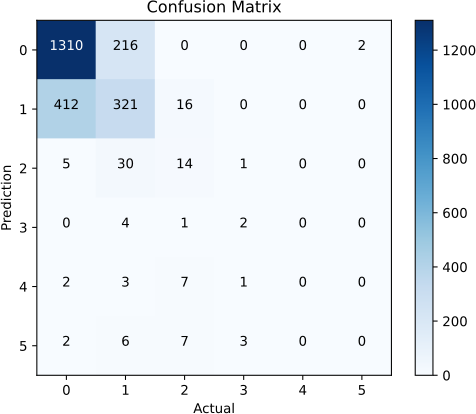
\includegraphics[width=\linewidth]{pics/confusion_matrix.png}
        \caption{Die exakte Konfusionsmatrix mit absoluten werten (Anzahl Gelenke).}
    \end{subfigure}
    \hfill
    \begin{subfigure}{0.45\textwidth}
        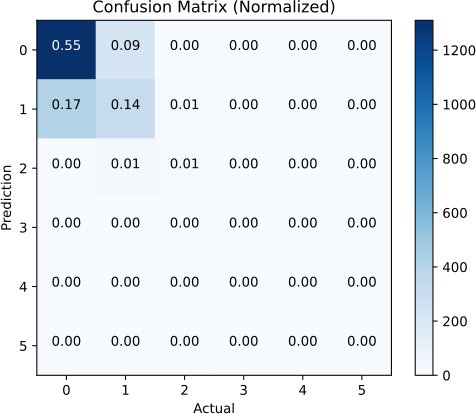
\includegraphics[width=\linewidth]{pics/confusion_matrix_norm.png}
        \caption{Die exakte Konfusionsmatrix normalisiert.}
    \end{subfigure}
    \par\bigskip
    \begin{subfigure}{0.45\textwidth}
        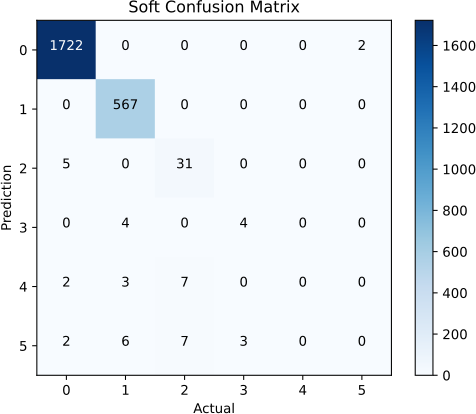
\includegraphics[width=\linewidth]{pics/soft_confusion_matrix.png}
        \caption{Die «weiche» Konfusionsmatrix mit absoluten werten (Anzahl Gelenke).}
    \end{subfigure}
    \hfill
    \begin{subfigure}{0.45\textwidth}
        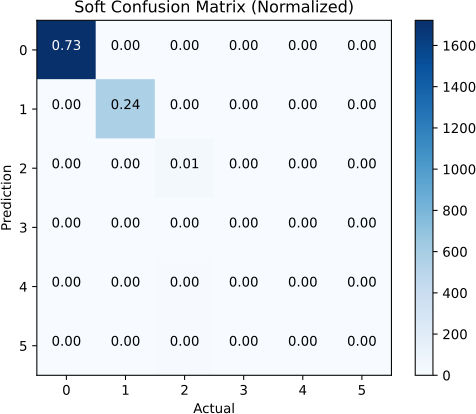
\includegraphics[width=\linewidth]{pics/soft_confusion_matrix_norm.png}
        \caption{Die «weiche» Konfusionsmatrix normalisiert.}
    \end{subfigure}
    \caption{Die verschiedenen Konfusionsmatrizen im Überblick.}
    \label{fig:konfusionsmatrizen}
\end{figure}

\subsubsection{Ergebnisse der Evaluation}

Die Evaluationsmetriken können mit einem Python-Skript berechnet und ausgegeben werden.\footnote{Siehe \texttt{deepxray/evaluation/evaluation/evaluation.py}. Die Ausgabe des Skripts ist in der Datei \texttt{evaluation/evaluation/evaluation.txt} zu finden.} Dabei werden folgende Ergebnisse ermittelt:

Die \textit{Global Accuracy} beträgt nach exaktem Vergleich $69.641\%$. Kommt Soft Matching zum Einsatz, beträgt sie $94.089\%$.

Die Ergebnisse der Metriken, die nach Klasse ermittelt werden, sind in \tblref{tbl:classaccuracies}; diejenigen, die auf \textit{Cohen's Kappa} basieren, in \tblref{tbl:cohenskappa} dargestellt.

\begin{table}[tbh]
    \center
    \begin{tabular}{l|l}
        Metrik & Ergebnis \\ \hline
        Class Accuracy (exakt) & $[0: 0.86, 1: 0.43, 2: 0.28, 3: 0.29, 4: 0.00, 5: 0.00]$ \\
        Class Accuracy (soft) & $[0: 0.99, 1: 0.98, 2: 0.69, 3: 0.57, 4: nan, 5: 0.00]$ \\
        Precision (exakt) & $[0: 0.86, 1: 0.43, 2: 0.28, 3: 0.29, 4: 0.00, 5: 0.00]$ \\
        Precision (soft) & $[0: 1.00, 1: 1.00, 2: 0.86, 3: 0.50, 4: 0.00, 5: 0.00]$ \\
        Recall (exakt) & $[0: 0.76, 1: 0.55, 2: 0.31, 3: 0.29, 4: nan, 5: 0.00]$ \\
        Recall (soft) & $[0: 0.99, 1: 0.98, 2: 0.69, 3: 0.57, 4: nan, 5: 0.00]$ \\
        F1-Score (exakt) & $[0: 0.80, 1: 0.48, 2: 0.29, 3: 0.29, 4: nan, 5: nan]$ \\
        F1-Score (soft) & $[0: 1.00, 1: 0.99, 2: 0.77, 3: 0.53, 4: nan, 5: nan]$ \\
    \end{tabular}
    \caption{Die Ergebnisse der klassenbasierten Evaluationsmetriken.}
    \label{tbl:classaccuracies}
\end{table}

\begin{table}[tbh]
    \center
    \begin{tabular}{l|r|r}
        Metrik & Ergebnis & Vertrauensintervall ($95\%$) \\ \hline
        Cohen's Kappa (exakt) & $0.324$ & $[0.283, 0.365]$ \\
        Cohen's Kappa (soft) & $0.957$ & $[0.945, 0.970]$ \\
        Cohen's Quadratic Kappa (exakt) & $0.449$ & $[0.443, 0.454]$ \\
        Cohen's Quadratic Kappa (soft) & $0.797$ & $[0.794, 0.801]$ \\
    \end{tabular}
    \caption{Die Ergebnisse der Evaluationsmetriken, die auf \textit{Cohen's Kappa} basieren.}
    \label{tbl:cohenskappa}
\end{table}

\subsubsection{Interpretation der Evaluationsergebnisse}

Bei den Konfusionsmatrizen (\imgref{fig:konfusionsmatrizen}) fällt auf, dass sich die Scores auf die beiden Klassen 0 (ca. $72\%$) und 1 (ca. $25\%$) konzentrieren. Vor diesem Hintergrund ist eine \textit{abschliessende} Interpration der Ergebnisse nicht angebracht. Für diese wären weitere Evaluationsdaten zu sammeln und zu verarbeiten. Dennoch können aus den verschiedenen Metriken einige Erkenntnisse gewonnen werden.

Die \textit{Global Accuracy} ist mit ca. $70\%$ (exakt) bzw. ca $94\%$ (soft) zwar hoch, aufgrund der unbalancierten Daten jedoch nicht aussagekräftig.\footnote{Hat die Mehrheit der Datenpunkte die Score 0, erreichte man mit einer statischen Prediction von 0 bereits eine Accuracy von über $50\%$.}

Bei den klassenbasierten Metriken fällt auf, dass für die Scores 4 und 5 keine Aussagen möglich sind. Tatsächlich lassen sich im Ergebnisdatensatz des Scorings nur zwei Gelenke mit der Score 5 und kein einziges der Score 4 finden.\footnote{Dies ist nicht \textit{nur} auf die \textit{false negatives} von \texttt{body\_part} zurückzuführen. So finden sich im ganzen Evaluationsdatensatz nur vier Gelenke der Score 4 und zwei der Score 5 (siehe Python-Skript \texttt{deepxray/test\_data/high\_scores.py}). Falsche Scores können auch auf eine fehlerhafte Gelenkextraktion hindeuten, zumal stark geschädigte Gelenke teilweise nicht mehr als solche zu erkennen sind.} Bei den Klassen von 0-3 fällt auf, dass die Übereinstimmungen bei den \textit{Soft Matches} durchgehend bedeutend höher ausfallen als diejenigen auf Basis exakter Vergleiche. Weiter gilt (mit wenigen geringfügigen Ausnahmen): Je höher die Score, desto unpräziser fallen die Predictions aus. Das könnte damit zu tun haben, dass die wenigen höheren Scores (Klassen 2 und 3) eher zufällig als systematisch übereinstimmen. Die \textit{Soft Matches} zeichnen hier ein etwas positiveres Bild, so beträgt die Übereinstimmung in den Klassen von 0 bis 3 zwischen $50\%$ und $100\%$ (gerundet).

Auch die Metriken \textit{Cohen's Kappa} und \textit{Cohen's Quadratic Kappa} hinterlassen einen gemischten Eindruck im Bezug auf die Performance. Diese fallen mit $0.324$ bzw. $0.449$ zu tief aus, dass der klinische Einsatz des Prototypen auch nur in Erwägung gezogen werden könnte.\footnote{\textit{«Any kappa below 0.60 indicates inadequate agreement among the ratorers and little confidence should be placed in the study results.»} \cite{interrater-reliability} Jedes Kappa unter 0.60 weist auf eine inadäquate Übereinstimmung unter den Bewertern hin, diesen Studienergebnissen sollte nur geringes Vertrauen entgegengebracht werden. (Übersetzung des Autors)}

Dass \textit{Cohen's Quadratic Kappa} grösser ausfällt als \textit{Cohen's Kappa} (jeweils in der exakten Variante), mag zunächst überraschen. Dies ist jedoch ein bekanntes statistisches Phänomen bei sogenannten \textit{tridiagonalen Tabellen}. Eine rechteckige Matrix (z.B. eine Konfusionsmatrix) ist tridiagonal, wenn nur in der Hauptdiagonalen (Übereinstimmungen) und in den beiden benachbarten Diagonalen (Sub- und Superdiagonalen) Werte auftauchen, die sich von null unterscheiden. Da es sich bei der Konfusionsmatrix in der vorliegenden Evaluation annähernd um eine tridiagonale Matrix handelt\footnote{Die Soft Matches, welche in den Haupt-, Sub- und Superdiagonalen zu liegen kommen, liegen ja weit über 90\%.}, ist der Unterschied zwischen den beiden Kappa-Metriken durchaus plausibel \cite{warrens-kappa}.

Auf Basis der \textit{Soft Matches} fallen die Kappas mit $0.957$ bzw. $0.797$ wesentlich höher aus. Dies könnte dahingehend interpretiert werden, dass der Prototyp zwar nicht sechs Klassen zuverlässig auseinanderhalten kann, jedoch in seinen Predictions nur geringfügige Abweichungen aufweist und immerhin für eine Unterscheidung zwischen tiefer, mittlerer und hoher Schädigung zuverlässig arbeitet. Aufgrund der Datenbasis mit sehr wenigen Daten in den höheren Klassen ist diese Interpretation jedoch voreilig.

\subsubsection{Anmerkung zu Soft Matches}
\label{sec:anmerkung-zu-soft-matches}

Die Soft Matches sind mit Vorsicht zu geniessen. Die menschlichen Scores liegen oft auf den Klassengrenzen der Predictions, z.B. liegt 20\% gerade auf der Grenze zwischen Klasse 1 ($]0\%..20\%]$) und 2 ($]20\%.. 40\%]$), gehört per Definition aber zur Klasse 1 \cite[S. 10]{rohrbach2017}. Somit sollte eine maschinelle Prediction legitimerweise den Scores 1 oder 2 zugeordnet werden ‒ zu 0 ($0\%$) und 3 ($]40\%..60\%]$) jedoch besser nicht. Die Soft-Match-Logik interpretiert jedoch nicht nur eine Score von 1 und 2, sondern auch von 0 als Übereinstimmung mit 20\%. Was bei einer menschlichen Score von 10\% durchaus sinnvoll wäre, schiesst bei Grenzfällen wie 20\% übers Ziel hinaus. Die Soft Matches arbeiten somit tendenziell zu grosszügig.

Um solche Grenzfälle in der Evaluation präziser behandeln zu können, müsste der Evaluationsworkflow Gebrauch der exakten menschlichen Scores machen. So könnte die \textit{Soft Confusion Matrix} beispielsweise für 10\% die Klassen 0, 1 und 2 als Treffer werten, für 20\% hingegen nur die Klassen 1 und 2. Dies dürfte zu präziseren ‒ und wohl etwas schlechter ausfallenden ‒ Soft-Metriken führen. Dieser erweiterte Evaluationsworkflow soll jedoch nicht im Rahmen der vorliegenden Arbeit umgesetzt werden.\footnote{Hierbei handelt es sich um einen klassischen Zielkonflikt: Der Data Miner möchte möglichst viele Daten zur Verfügung haben ‒ der Datenschützer möchte nur diejenigen zur Verfügung stellen, die für den jeweiligen Zweck unbedingt nötig sind. Der Projektmanager hingegen drängt auf den Abschluss der Evaluation, da noch eine Dokumentation zu schreiben ist.}

Die Toleranz der Abweichung könnte zudem empirisch bestimmt werden, indem die Abweichungen verschiedener menschlicher Scorer berücksichtigt werden. Hierfür stehen jedoch wissenschaftlich fundierte Metriken zur Verfügung (Stichwort \textit{Interclass Correlation}, ICC), sodass man vom Soft-Matching-Ansatz wegkommen könnte, stünden die Ergebnisse mehrerer menschlicher Scorer zur Verfügung.

\subsubsection{Fazit}

Der Evaluationsdatensatz ist unzureichend, um eine verbindliche Evaluation des Prototypen vornehmen zu können. Zwar weisen die Predictions für die tieferen Scores eine hohe Übereinstimmung auf, und die Abweichungen fallen betraglich eher gering aus. Für die höheren Klassen gibt es aber nur vereinzelte Datenpunkte, die keine signifikante Aussage zur Performance zulassen.

Wichtiger als ein solches Gesamturteil ist jedoch die Tatsache, dass ein weitgehend automatisierter Evaluationsworkflow mit verschiedenen Metriken umgesetzt worden ist, der in Zukunft mit weiteren Daten gefüttert und erneut ausgeführt werden kann. Schliesslich ist das Ziel der Evaluation nicht nur, eine einmalige Einschätzung des Systems vorzunehmen, sondern eine Möglichkeit zu haben, systematische Vergleiche zwischen verschiedenen Versionen des Systems anstellen zu können.

Für künftige Evaluationen ist zu beachten, dass neue und für Modellverbesserungen verwendete Trainingsdaten nicht mehr in der darauffolgenden Evaluation verwendet werden sollten.

\clearpage

\subsection{Evaluation der Zielerreichung}
\label{sec:evaluation-der-zielerreichung}

An dieser Stelle soll überprüft werden, ob und wie die Projektziele (siehe \secref{sec:erwartetes-resultat}) erreicht worden sind. Dies sind:

\begin{enumerate}
    \item \textit{Stand der Technik zur Industrialisierung (Evaluation, Testing) von ML-Modellen:} Dieses Thema wurde im Abschnitt \secref{sec:evaluation-von-modellen} auf Basis verschiedener Publikationen untersucht.
    \item \textit{Vorschlag für ein generisches Format von Modellen zum Exportieren aus ML-Frameworks und zum Importieren zur Ausführung:} Diese Problematik wurde in Abschnitt \secref{sec:modellformate} behandelt. Mittelfristig dürfte das SavedModel-Format von TensorFlow besser geeignet sein als das Format der ONNX-Initiative.
    \item \textit{Vorschlag für geeignete Metriken zum Vergleich von Modellen:} Hierzu wurden allgemeine Metriken (Accuracy, Precision, Recall, F1-Score) als auch domänenspezifische (Cohen's Kappa) gefunden (siehe \secref{sec:evaluationsmetriken}).
    \item \textit{Aufzeigen, was für eine Verheinheitlichung der Codebasis gemacht werden muss}: Diese Fragestellung wird im Ausblick behandelt (siehe \secref{sec:aktualisierung-auf-aktuelle-versionen}).
    \item \textit{Lauffähiger Prototyp}: Der Prototyp funktioniert und ist im Kapitel \secref{sec:realisierung} ausführlich dokumentiert.
    \begin{enumerate}
        \item \textit{Automatisierte Evaluation und Testing von neuen Modellen mit Vergleich zu alten Modellen und Minimum-Standards}: Der Evaluationsworkflow wurde umgesetzt, mit einem Evaluationsdatenset durchgeführt und ist in Abschnitt \secref{sec:technische-evaluation} dokumentiert.
        \item \textit{Visualisierung und Reporting der Performanz neuer Modelle}: Die Performanz kann über den Evaluationsworkflow (siehe wiederum \secref{sec:technische-evaluation}) ausgewertet werden. Als Visualisierung dienen verschiedene Konfusionsmatrizen (siehe \imgref{fig:konfusionsmatrizen}). Ein zusätzlich erstelltes Histogramm ist leider nur wenig aussagekräftig.
        \item \textit{API zum Ausführen des Modelles (Verteilen über mehrere GPUs)}: Die verschiedenen Modellkomponenten interagieren über eine Schnittstelle, die in Kapitel \secref{sec:realisierung} dokumentiert und auf \tblref{tbl:schnittstellen} übersichtlich zusammengefasst ist. Die Verteilung auf mehrere GPUs wurde nicht unternommen, da bereits mit CPUs eine akzeptable Performance erreicht werden konnte.
        \item \textit{Load Balancing, Messaging Systems}: Diese Thematik wurde in der Architekturdiskussion (\secref{sec:architekturvarianten}) ausführlich behandelt. Die verschiedenen Varianten für Messaging-Systeme werden kurz im Anhang evaluiert (siehe \secref{sec:wahl-der-message-queue}).
        \item \textit{Nahtloses Austauschen von alten Modellen mit neuen Versionen}: Die Austauschbarkeit kann nicht auf Modellebene, jedoch auf der Ebene der Modell\textit{komponenten} gewährleistet werden. Die Schnittstellen sind in \tblref{tbl:schnittstellen} zu finden.
    \end{enumerate}
\end{enumerate}

Fazit: Die wichtigsten Projektziele konnten erreicht werden. Dass die Austauschbarkeit der Machine-Learning-Modelle nicht auf Modellebene stattfinden konnte, zeichnete sich schon früh im Projektverlauf ab. Entsprechend wurde der Fokus früh auf die Austauschbarkeit von Modellkomponenten über definierte Schnittstellen gelegt. Im Bereich Visualisierung/Reporting wurde vergleichsweise wenig Aufwand investiert. Dafür musste zusätzliche Zeit investiert werden, um ein Modell neu zu trainieren, wofür die Modelldaten nicht mehr aufzufinden waren. Auch das Selektieren und Aufbereiten der Evaluationsdaten verursachte zusätzlichen Aufwand.

\subsubsection{Rückblick auf Projektrisiken}

Die zu Beginn des Projekts aufgestellten Projektrisiken (siehe \secref{sec:projektrisiken}) sollen an dieser Stelle wieder aufgegriffen werden. Sind Risiken eingetreten, und wenn ja, welchen Einfluss hatte dies auf den Projektverlauf? Haben sich die vorgeschlagenen Mitigationsmassnahmen als sinnvoll erwiesen?

\begin{description}
    \item[Keine lauffähigen Modelle] Dieses Risiko ist teilweise eingetreten, denn die Modelldaten zum \texttt{ratingen\_score}-Modell waren nicht mehr auffindbar. Die Mitigationsmassnahme, das Modell neu zu trainieren, konnte den Schaden eingrenzen. Dabei ist zwar Mehraufwand entstanden, das Projekt wurde dadurch aber nur unwesentlich verzögert.
    \item[Aktualisierung der Modelle] Dieses Risiko ist eingetreten, sodass die Aktualisierung der Modelle schon früh im Projektverlauf aufgegeben worden ist. Die Mitigationsmassnahmen (Isolation der bestehenden Modelle) haben sich als zielführend erwiesen. Der Prototyp konnte auf Basis der bestehenden Modelle umgesetzt werden.
    \item[Schlechte Performance (Prediction)] Die technische Evaluation lässt hier (noch) kein eindeutiges Urteil zu. Die Predictions bewegen sich ganz klar nicht im reinen Zufallsbereich, dürften aber für einen Produktiveinsatz noch zu wenig präzise sein. Dieses Risiko wird vom Auftraggeber getragen.
    \item[Schlechte Performance (Laufzeit)] Die Verarbeitungsgeschwindigkeit des Prototypen ist akzeptabel, wenn auch nicht berauschend. Die Anwendung ist skalierbar, sodass sich Hardwareerweiterungen (zusätzliche CPUs) und -verbesserungen (schnellere CPUs) positiv auf die Performance auswirken dürften.
    \item[Hoher Arbeitsspeicherverbrauch] Das Gesamtsystem benötigt mindestens 2 GB Arbeitsspeicher (eine Instanz pro Modellkomponente). Empfohlen sind 6 GB oder besser 11 GB (für fünf bzw. zehn laufende Instanzen der Gelenkextraktion). Diese Anforderungen stellen angesichts gegenwärtiger Speicherpreise kein Problem dar. Der Speicherbedarf ist jedoch kritisch, wenn die Modelle auf einer oder mehreren GPUs ausgeführt werden sollen.
\end{description}

Auf die Risiken, die für die einzelnen Projektphasen ermittelt worden sind (siehe \secref{sec:projektphasen}), soll an dieser Stelle nicht weiter eingegangen werden. Diese wurden jeweils ‒ falls nötig ‒ in der Reflexion der einzelnen Projektphasen kurz behandelt.

Obwohl einige der ermittelten Projektrisiken eingetreten sind, wurde der Erfolg des Projekts dadurch nicht beeinträchtigt. Die Mitigationsmassnahmen haben sich als sinnvoll und ausreichend erwiesen.
